\documentclass[tikz]{standalone}

\usetikzlibrary{arrows}
\usetikzlibrary{arrows.meta}

\begin{document}

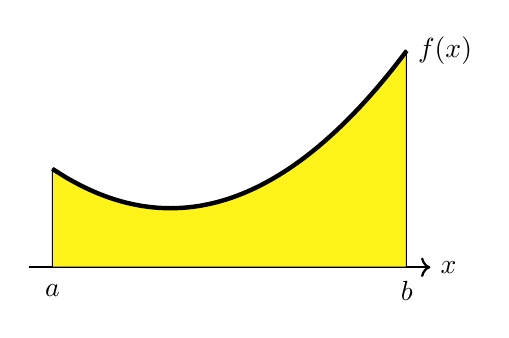
\begin{tikzpicture}[xscale=3,yscale=3.0]
    \draw[thick,->] (-0.6,0) -- (1.1,0) node[right] {$x$};
    \node at (-0.5, -0.1){$a$};
    \node at (1, -0.1) {$b$};
    \draw[fill=yellow!90] (-0.5,0) -- plot[smooth, samples=100, domain=-0.5:1 ] (\x,\x*\x/1.5 + 0.25) |- (-0.5,0);
    \draw[ultra thick,domain=-0.5:1,smooth,variable=\x,black] plot (\x,\x*\x/1.5 + 0.25) node[right]{$f(x)$};
  \end{tikzpicture}
  
  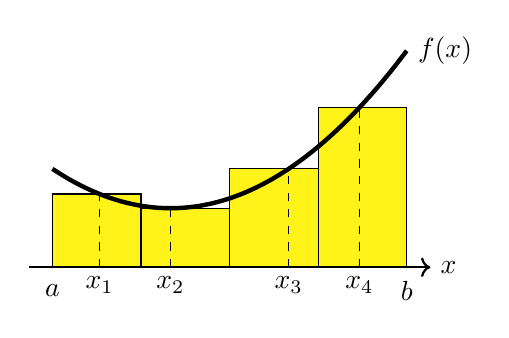
\begin{tikzpicture}[xscale=3,yscale=3.0]
    \node at (-0.5, -0.1){$a$};
    \node at (1, -0.1) {$b$};
  
    \draw[fill=yellow!90] (-0.5,0) rectangle ++(0.375,{(-0.3)^2 / 1.5 + 0.25});
    \draw [dashed] (-0.3,0) node[below] {$x_1$} -- (-0.3,{(-0.3)^2 / 1.5 + 0.25});
  
    \draw[fill=yellow!90] (-0.125,0) rectangle ++(0.375,{(0.0)^2 / 1.5 + 0.25});
    \draw [dashed] (0.0,0) node[below] {$x_2$} -- (0.0,{(0.0)^2 / 1.5 + 0.25});
          
    \draw[fill=yellow!90] (0.250,0) rectangle ++(0.375,{(0.5)^2 / 1.5 + 0.25});
    \draw [dashed] (0.5,0) node[below] {$x_3$} -- (0.5,{(0.5)^2 / 1.5 + 0.25});
  
    \draw[fill=yellow!90] (0.625,0) rectangle ++(0.375,{(0.8)^2 / 1.5 + 0.25});
    \draw [dashed] (0.8,0) node[below] {$x_4$} -- (0.8,{(0.8)^2 / 1.5 + 0.25});
          
    \draw[thick,->] (-0.6,0) -- (1.1,0) node[right] {$x$};
    \draw[ultra thick,domain=-0.5:1,smooth,variable=\x,black] plot (\x,\x*\x/1.5 + 0.25) node[right]{$f(x)$};
  
  \end{tikzpicture}


  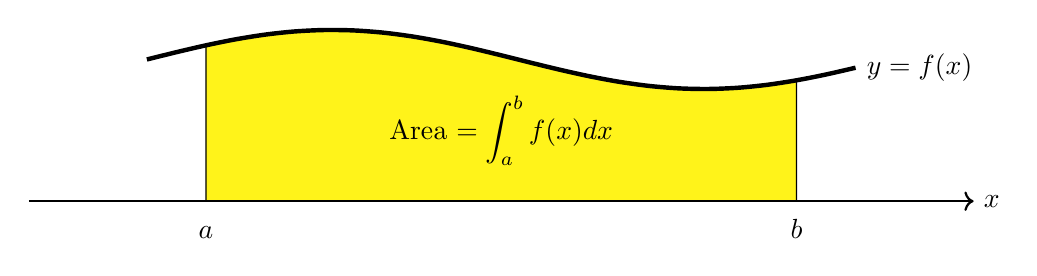
\begin{tikzpicture}[scale=1.5]

    % shade region
    \draw[fill=yellow!90,domain=0.5:5.5,smooth,variable=\x] (0.5,0) -- plot ({\x},{1.2 + 0.25*sin(\x r)}) |- cycle;
  
    % draw axis
    \draw[thick,->] (-1,0) -- (7,0) node[right] {$x$};
  
    % draw curve
    \draw[ultra thick,domain=0:6,smooth,variable=\x,black] plot ({\x},{1.2 + 0.25*sin(\x r)}) node[right]{$y=f(x)$};
  
    \node at (0.5, -0.4) [above] {$a$};
    \node at (5.5, -0.4) [above] {$b$};      
          
    \node at (3, 0.6) {Area $ = \displaystyle \int_a^b f(x)dx$};
  \end{tikzpicture}

  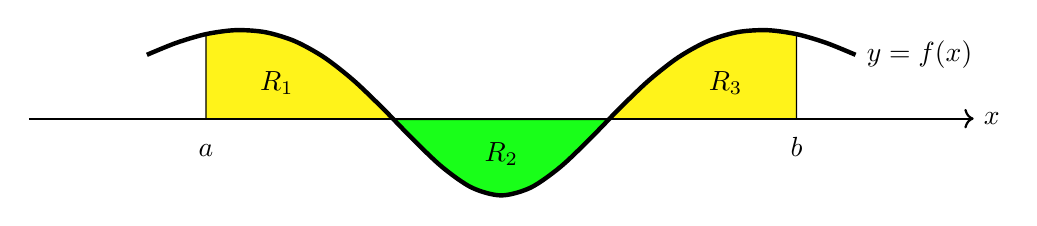
\begin{tikzpicture}[scale=1.5]

    % shade region
    \draw[fill=yellow!90,domain=0.5:5.5,smooth,variable=\x] (0.5,0) -- plot ({\x},{0.05 - 0.7*cos(1.8*0.9^(abs(\x-3))*(\x - 3.0) r)}) |- cycle;
  
    \draw[fill=green!90,domain=2.09:3.91,smooth,variable=\x] plot ({\x},{0.05 - 0.7*cos(1.8*0.9^(abs(\x-3))*(\x - 3.0) r)}) -- cycle;
  
    % draw axis
    \draw[thick,->] (-1,0) -- (7,0) node[right] {$x$};
  
    % draw curve
    \draw[ultra thick,domain=0:6,smooth,variable=\x,black] plot ({\x},{0.05 - 0.7*cos(1.8*0.9^(abs(\x-3))*(\x - 3.0) r)}) node[right]{$y=f(x)$};
  
    \node at (1.1, 0.3) {$R_1$};
    \node at (3, -0.3) {$R_2$};
    \node at (4.9, 0.3) {$R_3$};
  
    \node at (0.5, -0.4) [above] {$a$};
    \node at (5.5, -0.4) [above] {$b$};      
  \end{tikzpicture}

  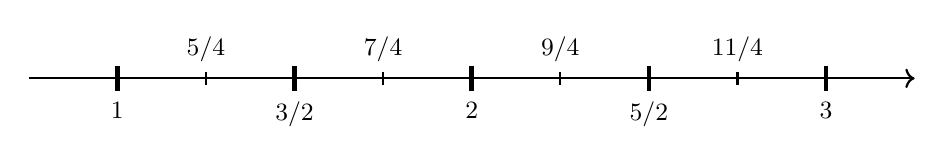
\begin{tikzpicture}[baseline=-0.5ex,scale=4.5]
    \draw[thick,->] (0.75,0) -- (3.25,0);
    \foreach \x in {1, 2, 3}{
      \draw [ultra thick] (\x cm,1.0pt) -- (\x cm,-1.0pt) node[below]{\small$\x$};
    }
    \foreach \x in {3, 5}{
      \draw [ultra thick] (0.5*\x cm,1.0pt) -- (0.5*\x cm,-1.0pt) node[below]{\small$\x/2$};
    }
    \foreach \x in {5, 7,9,11}{
      \draw [thick] (0.25*\x cm,-0.5pt) -- (0.25*\x cm,0.5pt) node[above]{\small$\x/4$};
    }
  \end{tikzpicture}

  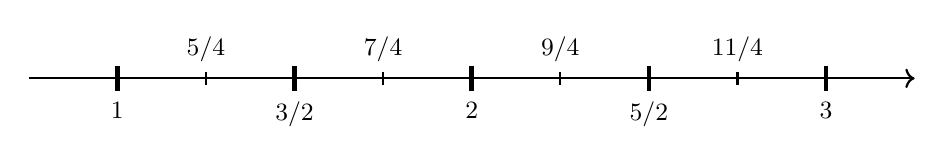
\begin{tikzpicture}[baseline=-0.5ex,scale=4.5]
    \draw[thick,->] (0.75,0) -- (3.25,0);
    \foreach \x in {1, 2, 3}{
      \draw [ultra thick] (\x cm,1.0pt) -- (\x cm,-1.0pt) node[below]{\small$\x$};
    }
    \foreach \x in {3, 5}{
      \draw [ultra thick] (0.5*\x cm,1.0pt) -- (0.5*\x cm,-1.0pt) node[below]{\small$\x/2$};
    }
    \foreach \x in {5, 7,9,11}{
      \draw [thick] (0.25*\x cm,-0.5pt) -- (0.25*\x cm,0.5pt) node[above]{\small$\x/4$};
    }
  \end{tikzpicture}

  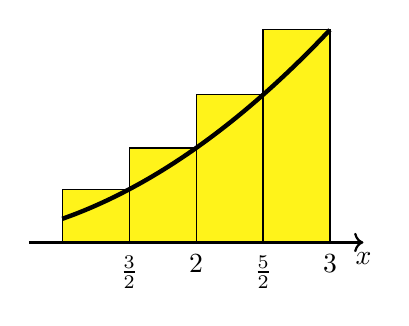
\begin{tikzpicture}[xscale=1.7,yscale=0.3]

    % create a white background, with a black frame
    % \draw [fill=white] (0.6,-3) rectangle (3.4,10); 
  
    % draw Riemann Sum - Right Riemann sum 
    \foreach \x in { 1,1.5,2,2.5} {
      \draw [fill=yellow!90] (\x,0) rectangle +(0.5,{(\x+0.5)*(\x+0.5)});
    }
  
    % draw axes
    \draw [->,thick] (0.75,0) -- (3.25,0) node[below] {$x$}; 
  
    % tick marks
    \foreach \x in {2,3} 
      \draw [thick] (\x cm,2pt) -- (\x cm,-2pt) node[below] {\x};
    \foreach \x in {3, 5}{
      \draw [ultra thick] (0.5*\x cm,2pt) -- (0.5*\x cm,-2pt) node[below]{$\frac{\x}{2}$};
      }
  
    % plot function
    \draw [ultra thick,smooth,variable=\x] plot [domain=1:3] (\x,\x*\x);
  
  \end{tikzpicture}

  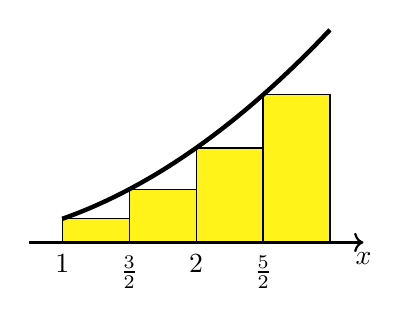
\begin{tikzpicture}[xscale=1.7,yscale=0.3]

    % create a white background, with a black frame
    % \draw [fill=white] (0.6,-3) rectangle (3.4,10); 
  
    % draw Riemann Sum - Left Riemann sum 
    \foreach \x in { 1,1.5,2,2.5} {
      \draw [fill=yellow!90] (\x,0) rectangle +(0.5,{(\x+0)*(\x+0)});
    }
  
    % draw axes
    \draw [->,thick] (0.75,0) -- (3.25,0) node[below] {$x$}; 
  
    % tick marks
    \foreach \x in {1,2} 
      \draw [thick] (\x cm,2pt) -- (\x cm,-2pt) node[below] {\x};
    \foreach \x in {3, 5}{
      \draw [ultra thick] (0.5*\x cm,2pt) -- (0.5*\x cm,-2pt) node[below]{$\frac{\x}{2}$};
      }
  
    % plot function
    \draw [ultra thick,smooth,variable=\x] plot [domain=1:3] (\x,\x*\x);
  
  \end{tikzpicture}

  
  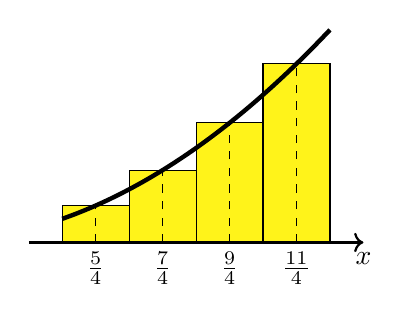
\begin{tikzpicture}[xscale=1.7,yscale=0.3]

    % create a white background, with a black frame
    % \draw [fill=white] (0.6,-3) rectangle (3.4,10); 
  
    %% draw a grid
    %\draw[step=2mm, lightgray, thin] (-0.5,-0.7) grid (5.5,1.99); 
    %\draw[step=1cm, gray] (-0.5,-0.7) grid (5.5,1.99); 
  
    % draw Riemann Sum - Midpoint rule 
    \foreach \x in { 1,1.5,2,2.5} {
      \draw [fill=yellow!90] (\x,0) rectangle +(0.5,{(\x+0.25)*(\x+0.25)});
    }
  
    % draw axes
    \draw [->,thick] (0.75,0) -- (3.25,0) node[below] {$x$}; 
  
    % tick marks
    \foreach \x in {5, 7,9,11}{
      \draw [thick] (0.25*\x cm,-1pt) -- (0.25*\x cm,1pt) node[below]{$\frac{\x}{4}$};
      \draw [dashed] (0.25*\x cm,0) -- (0.25*\x cm,\x*\x/16);
      }
  
    % plot function
    \draw [ultra thick,smooth,variable=\x] plot [domain=1:3] (\x,\x*\x);
  
  \end{tikzpicture}
  
\end{document} 